\chapter{Motor}
%vorstellen was in diesem Kapitel gesagt werden soll
%oder eher erklären bsp. Regeln von Motor von EEROS

%\section*{Stichworte}
%\begin{itemize}
%\item überblick (zusammen mit EEROS)
%\item Aufbau urdf
%\item verwendung von urdf
%\item gazebo plugins
%\item joint state publisher
%\item rqt plugins
%\end{itemize}

In diesem Kapitel wird anhand eines einfachen Fallbeispiels gezeigt, wie mit \textit{ROS} die Entwicklung einer \textit{EEROS} Applikation unterstützt werden kann. 
Das System ins diesem Fallbeispiel ist eine Motor"=Baugruppe (Abbildung \ref{Ab:motor-baugruppe}).

Für dieses System muss im \textit{EEROS} ein Regler entwickelt werden.
Um die Entwicklung zu unterstützen und den Regler zu testen, soll eine Simulation verwendet werden.
Und um die Leistung des Reglers besser beurteilen zu können sollen Plots von den zeit-variablen Grössen erstellt werden.

%Darum braucht es eine Simulation der Motor"=Baugruppe mit der der Regler getestet werden kann.
%Und auch eine Visualisierung mit der das Verhalten des Regler in einem Plot dargestellt werden kann.

%In diesem Kapitel wird anhand eines einfachen Fallbeispiels gezeigt, wie eine Simulation in Gazebo erstellt wird.
Durch das einfache Beispiel können alle Grundlagen vorgestellt werden, die es braucht um eine Simulation und die Visualisierungen zu erstellen.
%Ein Motor-Baugruppe (Abbildung \ref{Ab:motor-baugruppe}) soll als einfache Beispiel dienen.


\begin{figure}[ht!]
	\centering
	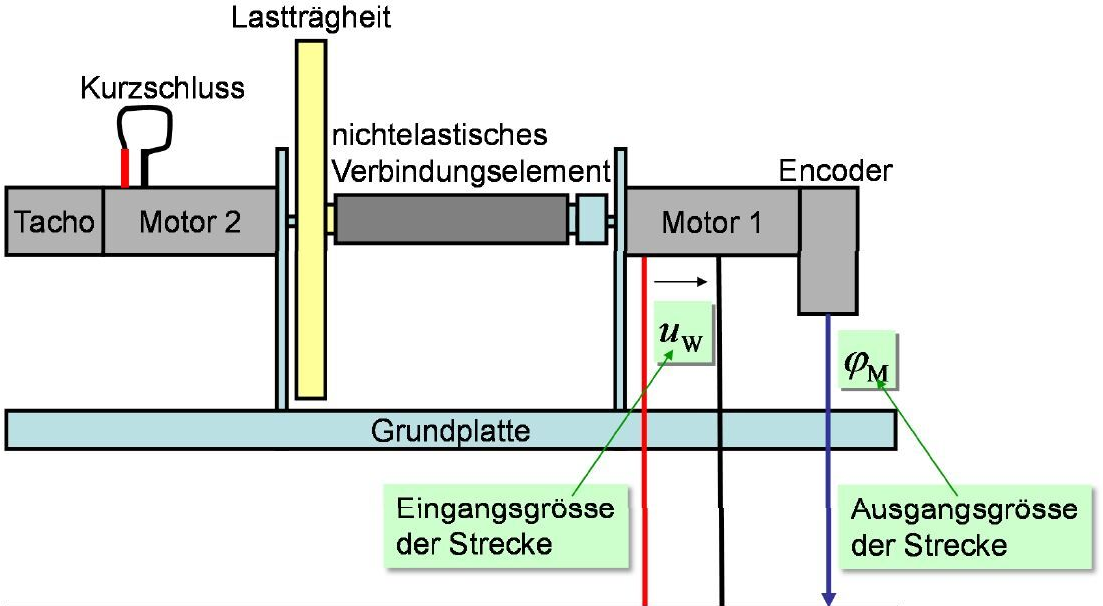
\includegraphics[width=14.5cm]{images/motor_baugruppe.png} %TODO anpassen
	\caption{Motor-Baugruppe}
	\label{Ab:motor-baugruppe}
\end{figure}

\section{Motor"=Baugruppe}
Die Baugruppe besteht aus einem Motor, Schwungrad und linearen Dämpfer.
Diese drei Komponenten sind mit einander verbunden.
Der lineare Dämpfer ist realisiert durch einen zweiten kurzgeschlossenen Motor.

Die Parameter für Simulations"=Model konnten grössten teils aus den Datenblättern der jeweiligen Komponenten entnommen werden. %TODO ref anhang / repo
Berechnung dämpfung
Für Parameter die nicht im Datenblatt stehen oder nicht genügend Informationen für eine Berechnung vorhanden ist, wurden geschätzt.
Jedoch haben die geschätzten Parameter in dieser Simulation keinen nennenswerten Einfluss.
%Somit haben wir folgende Werte die für die physikalische Beschreibung des Modells.
%Für jeden Link müssen immer die Masse und der Trägheits-tensor definiter sein. Dabei darf die Masse nicht 0 sein und %TODO abklären inertia = 0 

Auflistung von Parametern


\section{Gazebo}
\subsection{URDF}
nur Beispiel hier vom Link Dämpfer und vom joint Dämpfer Achse

erwähnen es könnten Vereinfachungen vom Model gemacht werden
jedoch hier bewusst nicht gemacht um Spezialfälle zu zeigen

bild tree structure

bild kin close


\subsection{Gazebo Plugins}
beschreiben für was die Plugins sind, wie sie eingesetzt werden
joint publisher


\subsubsection{Joint Force Plugin}
joint_force vorstellen

auf tutorial verweisen

es wird vor jedem Simulations"=Schritt aufgerufen

sync erklären

Fälle von Einsatz: 2 oder 3. auch noch

wie benutzen 


\section{rviz}
system wird geladen mit robot description
braucht auch tf

\subsection{Joint State Publisher}
erklären für was gebraucht wird

\section{rqt}
keine speziellen anpassungen an urdf 



